%
%% This is file `sample-manuscript.tex',
%% generated with the docstrip utility.
%%
%% The original source files were:
%%
%% samples.dtx  (with options: `manuscript')
%% 
%% IMPORTANT NOTICE:
%% 
%% For the copyright see the source file.
%% 
%% Any modified versions of this file must be renamed
%% with new filenames distinct from sample-manuscript.tex.
%% 
%% For distribution of the original source see the terms
%% for copying and modification in the file samples.dtx.
%% 
%% This generated file may be distributed as long as the
%% original source files, as listed above, are part of the
%% same distribution. (The sources need not necessarily be
%% in the same archive or directory.)
%%
%% The first command in your LaTeX source must be the \documentclass command.
%%%% Small single column format, used for CIE, CSUR, DTRAP, JACM, JDIQ, JEA, JERIC, JETC, PACMCGIT, TAAS, TACCESS, TACO, TALG, TALLIP (formerly TALIP), TCPS, TDSCI, TEAC, TECS, TELO, THRI, TIIS, TIOT, TISSEC, TIST, TKDD, TMIS, TOCE, TOCHI, TOCL, TOCS, TOCT, TODAES, TODS, TOIS, TOIT, TOMACS, TOMM (formerly TOMCCAP), TOMPECS, TOMS, TOPC, TOPLAS, TOPS, TOS, TOSEM, TOSN, TQC, TRETS, TSAS, TSC, TSLP, TWEB.
% \documentclass[acmsmall]{acmart}

%%%% Large single column format, used for IMWUT, JOCCH, PACMPL, POMACS, TAP, PACMHCI
% \documentclass[acmlarge,screen]{acmart}

%%%% Large double column format, used for TOG
% \documentclass[acmtog, authorversion]{acmart}

%%%% Generic manuscript mode, required for submission
%%%% and peer review
\documentclass[manuscript,screen,review]{acmart}
\usepackage{kotex}
\usepackage{graphicx}

\usepackage{array}
\usepackage{listings} 
\usepackage{xcolor} 
\usepackage{algorithm}
\usepackage{algpseudocode}

\definecolor{codegreen}{rgb}{0,0.6,0} 
\definecolor{codegray}{rgb}{0.5,0.5,0.5} 
\definecolor{codepurple}{rgb}{0.58,0,0.82} 
\definecolor{backcolour}{rgb}{0.95,0.95,0.92}

\renewcommand{\abstractname}{}
\newcommand{\factorial}{\ensuremath{\mbox{\sc Factorial}}}

\lstdefinestyle{mystyle}{ 
	backgroundcolor=\color{backcolour},
	commentstyle=\color{codegreen},
	keywordstyle=\color{magenta},
	numberstyle=\tiny\color{codegray},
	stringstyle=\color{codepurple},
	basicstyle=\ttfamily\footnotesize,
	breakatwhitespace=false,
	breaklines=true,
	captionpos=b,
	keepspaces=true,
	numbers=left,
	numbersep=5pt,
	showspaces=false,
	showstringspaces=false,
	showtabs=false,
	tabsize=2 
} 
\lstset{style=mystyle}
%%
%% \BibTeX command to typeset BibTeX logo in the docs
\AtBeginDocument{%
  \providecommand\BibTeX{{%
    \normalfont B\kern-0.5em{\scshape i\kern-0.25em b}\kern-0.8em\TeX}}}

%% Rights management information.  This information is sent to you
%% when you complete the rights form.  These commands have SAMPLE
%% values in them; it is your responsibility as an author to replace
%% the commands and values with those provided to you when you
%% complete the rights form.


%%
%% Submission ID.
%% Use this when submitting an article to a sponsored event. You'll
%% receive a unique submission ID from the organizers
%% of the event, and this ID should be used as the parameter to this command.
%%\acmSubmissionID{123-A56-BU3}

%%
%% The majority of ACM publications use numbered citations and
%% references.  The command \citestyle{authoryear} switches to the
%% "author year" style.
%%
%% If you are preparing content for an event
%% sponsored by ACM SIGGRAPH, you must use the "author year" style of
%% citations and references.
%% Uncommenting
%% the next command will enable that style.
%%\citestyle{acmauthoryear}

%%
%% end of the preamble, start of the body of the document source.
\begin{document}

%%
%% The "title" command has an optional parameter,
%% allowing the author to define a "short title" to be used in page headers.
\title{Sub45 final report}

%%
%% The "author" command and its associated commands are used to define
%% the authors and their affiliations.
%% Of note is the shared affiliation of the first two authors, and the
%% "authornote" and "authornotemark" commands
%% used to denote shared contribution to the research.
\author{이유섭}
\authornote{본 저자는 이 보고서를 쓰며 크게 성장했다.}
\email{lys7aves@naver.com}
\orcid{1234-5678-9012}
\authornotemark[1]
\affiliation{%
  \institution{Korea University}
  \streetaddress{서울특별시 성북구 안암로 고려대학교}
  \city{Seoul}
  \state{}
  \country{Korea}
  \postcode{02841}
}

%%
%% By default, the full list of authors will be used in the page
%% headers. Often, this list is too long, and will overlap
%% other information printed in the page headers. This command allows
%% the author to define a more concise list
%% of authors' names for this purpose.
\renewcommand{\shortauthors}{이유섭}

%%
%% The abstract is a short summary of the work to be presented in the
%% article.
\begin{abstract}
  본 보고서는 3*3 puzzle problem을 A* algorithm과 Iterative Deepening Search 두 알고리즘을 통해 푼 과정과 Autoregressive Model과 Gaussian Process을 이용한 Bitcoin 예측 과정에 대해 서술하였다.
\end{abstract}

%%
%% The code below is generated by the tool at http://dl.acm.org/ccs.cfm.
%% Please copy and paste the code instead of the example below.
%%
\begin{CCSXML}
<ccs2012>
 <concept>
  <concept_id>10010520.10010553.10010562</concept_id>
  <concept_desc>Computer systems organization~Embedded systems</concept_desc>
  <concept_significance>500</concept_significance>
 </concept>
 <concept>
  <concept_id>10010520.10010575.10010755</concept_id>
  <concept_desc>Computer systems organization~Redundancy</concept_desc>
  <concept_significance>300</concept_significance>
 </concept>
 <concept>
  <concept_id>10010520.10010553.10010554</concept_id>
  <concept_desc>Computer systems organization~Robotics</concept_desc>
  <concept_significance>100</concept_significance>
 </concept>
 <concept>
  <concept_id>10003033.10003083.10003095</concept_id>
  <concept_desc>Networks~Network reliability</concept_desc>
  <concept_significance>100</concept_significance>
 </concept>
</ccs2012>
\end{CCSXML}

\ccsdesc[500]{Computer systems organization~Embedded systems}
\ccsdesc[300]{Computer systems organization~Redundancy}
\ccsdesc{Computer systems organization~Robotics}
\ccsdesc[100]{Networks~Network reliability}

%%
%% Keywords. The author(s) should pick words that accurately describe
%% the work being presented. Separate the keywords with commas.
\keywords{sub45, 3*3 puzzle problem, A* algorithm, Iterative Deepening Search, Autoregressive Model, Gaussian Process, Bitcoin}


%%
%% This command processes the author and affiliation and title
%% information and builds the first part of the formatted document.
\maketitle

\section{3*3 puzzle problem}
\subsection{문제}

\begin{figure}[h] %%% t: top, b: bottom, h: here
\begin{center}
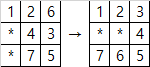
\includegraphics[width=0.5\linewidth]{33_puzzle.png}
\end{center}
\caption{3*3 puzzle}
\label{fig:long}
\label{fig:onecol}
\end{figure}

위의 퍼즐을 두 가지 알고리즘으로 풀어 성능비교 (속도 등)

\begin{itemize}
\item A* algorithm
\item Iterative Deepening Search
\end{itemize}

\subsection{선행연구들 요약 (literature review)}

\subsubsection{A* algorithm}\

A* algorithm은 출발 지점에서 목표 지점까지 최단 경로를 찾아내는 알고리즘 중 하나이다.
해당 알고리즘은 다익스트라 알고리즘과 유사하나 출발점에서 각 지점까지의 거리 뿐만 아니라 해당 지점에서 목표지점까지의 휴리스틱 추정값을 복합적으로 사용하여 경로를 찾는 알고리즘이다. 식은 다음과 같이 정리할 수 있다.
\begin{equation}
  f(n) = g(n) + h(n)
\end{equation}
\begin{itemize}
  \item g(n) : 출발 지점으로부터 지점 n까지의 길이
  \item h(n) : 지점 n으로부터 목표 지점까지의 추정 길이
\end{itemize}
h(n)의 값은 특별히 정해진 함수가 아니기 때문에 A* algorithm을 쓰더라도 h(n)을 어떻게 정의하느냐에 따라 그 결과가 달라진다.

\subsubsection{Iterative Deepening Search}\

Iterative Deepening Search(이하 IDS)는 DFS와 BFS의 단점들을 보완하기 위해 고안된 알고리즘이다. DFS는 사이클에 빠지거나 한번 길을 잘못 들면 매우 무한루프에 빠지거나 답을 구하기까지 매우 오랜 시간이 걸린다. 반면에 BFS는 optimal하게 경로를 구할 수 있지만 메모리 소모가 크다.

두 알고리즘의 단점을 보안한 IDS는 DFS의 작동 방식을 기반으로 한다. 그러나 기존의 DFS와 달리 탐색 깊이를 제한하여 무한루프에 빠지거나 잘못된 길에 들어섰을 때 빠르게 빠져 나올 수 있게 한다. 그러나 깊이를 제한하면 답을 찾지 못할 수도 있는데, 때문에 답을 찾을 때까지 깊이를 1부터 차례로 늘려나가면서 탐색을 한다. 이는 깊이를 1씩 늘려나가기 때문에 항상 optimal하게 경로를 구할 수 있으며, DFS의 메모리를 적게 사용한다는 장점까지 그대로 적용한 알고리즘이라고 할 수 있다.

\subsection{사용한 데이터}

문제에서 제시한 퍼즐을 데이터로 사용하였다.

\subsection{제안 알고리즘}

A* algorithm과 Iterative Deepening Search을 사용하여 3*3 puzzle problem을 해결하였다. 또한, 두 알고리즘의 성능을 비교하고자 하였는데, 각 알고리즘에서 데이터를 처리하는 방식이 미세하게 다르며, 직관적인 코딩을 위해 최적화를 시키지 않았다는 점 등 여러 원인에 의해 실제 알고리즘에서 추구하는 시간 복잡도와 달라질 수 있다는 점을 감안하여 성능 비교 시 지점 방문 횟수로 시간을 측정하였으며, 메모리는 반납된 메모리까지 고려하여 최대 메모리로 측정하였다.

\begin{lstlisting}[language=python, caption=main and init function] 
def main():
    [curr, goal] = init()
    AStarAlgorithm(curr, goal)
    IterativeDeepeningSearch(curr, goal)

def init():
    curr = [[1,2,6], ['*',4,3], ['*',7,5]]
    goal = [[1,2,3], ['*','*',4], [7,6,5]]
    return [curr, goal]
\end{lstlisting}

위의 코드는 main 함수와 init 함수가 어떻게 이루어졌는지에 대해 기술도어 있다. init 함수는 퍼즐의 현재 상태와 목표 상태를 만들어 반환해주는 함수이며, main 함수 실행 시, init함수를 호출하여 현재 상태와 목표 상태를 받고, 이를 AStarAlgorithm 함수와 IterativeDeepeningSearch 함수를 통해 A* algorithm과 IDS를 수행하였다.
AStarAlgorithm 함수와 IterativeDeepeningSearch함수는 뒤에 더 자세히 기술하였다.

\subsubsection{A* algorithm}\

A* 알고리즘에서 g(n)은 출발 지점으로부터 지점 n까지의 길이이기 때문에 지점 n까지 도달하기 위해 움직인 횟수로 정의할 수 있다. 그렇다면 h(n)은 어떻게 정의해야 할까? 다양한 방법이 있을 수 있지만, 본 보고서에서는 h(n)은 현재 퍼즐과 목표 퍼즐을 비교하였을 때, 각 숫자들의 택시 기하학에서의 직선 거리 합으로 정의하였다. 또한, 현재까지 구한 지점들의 함수값과 퍼즐 상태를 우선순위큐에 저장함으로써 다음으로 탐색할 지점을 빠르게 결정할 수 있도록 하였다.

다음은 A* algorithm을 구현한 AStarAlgorithm 함수이다.

\begin{lstlisting}[language=python, caption=AStarAlgorithm function] 
def AStarAlgorithm(curr, goal):
    start_time = time.time()
    print('----- start to A* alogrithm -----')
    curr = starToZero(curr)
    goal = starToZero(goal)
    puzzle_size = len(curr) * len(curr[0])
    
    que = PriorityQueue()
    que.put([0, curr, []])
    
    Time = 0
    memory = puzzle_size
    
    while(not que.empty()):
        Time = Time + 1
        memory = max(memory, que.qsize()*puzzle_size)
        
        [curr, path] = que.get()[1:3]
        if(curr == goal):
            print('find!')
            for puzzle in path:
                print(puzzle)
            break
        
        flag = False
        for i in range(len(curr)):
            for j in range(len(curr[0])):
                if(curr[i][j] == 0):
                    moves = Move(curr, i, j)
                    for move in moves:
                        if(move == curr):
                            continue
                        
                        distance = Distance(curr, goal)
                        
                        path_ = copy.deepcopy(path)
                        path_.append(move)
                        
                        que.put([distance+len(path), move, path_])
                
    print('A* Algorithm')
    print('time : ', Time)
    print('memory : ', memory)
    print('real time : ', time.time() - start_time)
    print()
    
    return [Time, memory]
\end{lstlisting}

starToZero 함수는 '*' 문자가 포함된 퍼즐의 상태를 우선순위 큐에 넣으면 대소 비교의 문제가 발생해 A* algorithm에 한에 '*' 문자를 숫자 0으로 바꿔 처리하였다.

노드(지점) 관리는 앞서 말했듯이 우선순위 큐를 이용하였으며, 시간은 우선순위 큐에서 pop을 한 횟수로 계산하였고, 메모리는 (우선순위 큐의 최대 크기)*(퍼즐의 크기)로 계산하였다.

Move(curr, i, j) 함수는 curr 상태의 퍼즐 중 (i, j) 블럭을 상하좌우를 상하좌우로 움직였을 때 나올 수 있는 퍼즐의 상태 리스트를 반환해주는 함수이다. i와 j의 값에 따라 움직이는게 무의미할 때도, 특정 방향으로 움직이지 못할 때도 있기 때문에 따로 함수를 이용해 작성하였다.

\subsubsection{Iterative Deepening Search}\

Iterative Deepening Search는 우선 limit가 존재하는 DFS 함수를 작성하고 limit를 1부터 순차적으로 증가시켜 가면서 DFS 함수를 호출함으로써 코드를 완성시킬 수 있다. 이때, 시간은 각 DFS 함수를 호출시켰을 때 나온 시간의 합으로 계산하였으며, 메모리는 특정 limit에 대한 DFS 함수가 종료되면 DFS 실행에 사용된 모든 메모리를 반납할 수 있기 때문에 메모리는 각 DFS 함수를 호출시켰을 때 나온 메모리의 최대값으로 계산하였다.

\begin{lstlisting}[language=python, caption=IterativeDeepeningSearch function] 
def IterativeDeepeningSearch(curr, goal):
    start_time = time.time()
    print('----- start to Iterative Deepening Search -----')
    Time = 0
    memory = 0
    
    limit = 0
    while(1):
        [Time_, memory_, flag] = DFS(curr, goal, 0, limit)
        
        Time = Time + Time_
        memory = max(memory, memory_)
        
        print(limit, Time, memory, flag)
        
        if(flag):
            break;
        
        limit = limit+1
        
    
                
    print('Iterative Deepening Search')
    print('time : ', Time)
    print('memory : ', memory)
    print('real time : ', time.time() - start_time)
    
    return [Time, memory]
\end{lstlisting}

DFS 함수는 현재 상태와 목표 상태, 깊이, 제한을 인자로 받아 DFS를 도는 함수이며, 반환값으로 DFS 함수 수행에 걸린 시간, 사용 메모리, 목표 지점까지 도달 여부를 반환하는 함수이다. 아래는 본 보고서에서 작성한 DFS 코드이다.

\begin{lstlisting}[language=python, caption=IterativeDeepeningSearch function] 
def IterativeDeepeningSearch(curr, goal):
def DFS(curr, goal, depth, limit):
    puzzle_size = len(curr) * len(curr[0])
    
    if(depth > limit):
        return [0, 0, False]
    if(curr == goal):
        return [1, puzzle_size, True]
    
    Time = 1
    memory = 0
    for i in range(len(curr)):
        for j in range(len(curr[0])):
            if(curr[i][j] == '*'):
                moves = Move(curr, i, j)
                for move in moves:
                    if(move == curr):
                        continue
                    [Time_, memory_, flag] = DFS(move, goal, depth+1, limit)
                    
                    Time = Time + Time_
                    memory = max(memory, memory_)
                    if(flag):
                        return [Time, memory+puzzle_size, True]
                    
    return [Time, memory+puzzle_size, False]
\end{lstlisting}

앞서 말했듯이, DFS에서 전체 탐색 시간은 자식들의 탐색시간의 합 + 1로 계산하였으며, 메모리는 자식들의 메모리의 최댓값 + 1로 계산하였다.

\subsection{실험 환경 및 실험}

3*3 puzzle problem 프로그램은 실험은 Ubuntu 20.04.1 LTS 환경에서 진행하였으며, ptyhon은 3.8.5 버전을 사용하였다.

아래는 위에서 언급한 환경에서 프로그램을 실행시킨 결과이다.

\begin{figure}[h] %%% t: top, b: bottom, h: here
\begin{center}
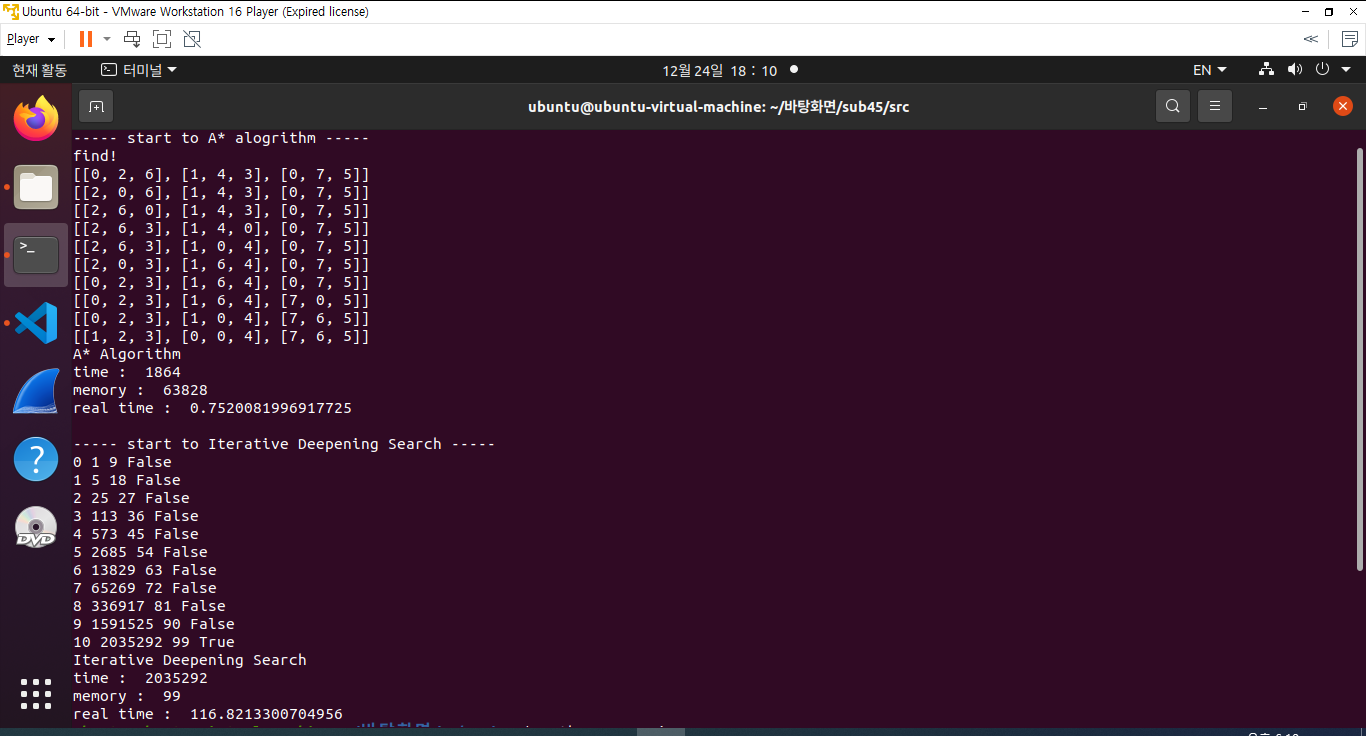
\includegraphics[width=1\linewidth]{result.PNG}
\end{center}
\caption{3*3 puzzle problem 프로그램 실행 결과}
\label{fig:long}
\label{fig:onecol}
\end{figure}

\subsection{정보보안과 연결시키기 - 응용분야 도출}

길찾기 알고리즘은 정보보안과 연결을 시키면 네트워크 역추적과 같이 추척이나 흐름 파악 등에 활용될 수 있을 것 같다. A* algorithm은 특정 패킷이 어디서 날아온 패킷인지 알고 싶을 때, 그 패킷이 온 곳을 따라가면서 추가로 패킷과 주변 네트워크와의 유사도를 이용하는 등으로 일반적인 BFS보다 빠르게 추척할 수 있을 것이며, IDS의 경우 회사 내부 트래픽과 같이 트래픽의 경로가 길지 않을 것이라고 추정되는 곳에서 네트워크 역추적에 적합할 것 같다.

\section{Autoregressive Model과 Gaussian Process을 이용한 Bitcoin 예측}

\subsection{문제}

2020년 11월의 Bitcoin 값을 일별로 추출하여 가격을 예측하는 프로그램을 만들어주세요. 특히, AR과 GP간의 성능(속도, 정확도)비교를 해주세요.

\subsection{선행연구들 요약 (literature review)}

\subsubsection{Autoregressive Model}\

Autoregressive Model(이하 AR model)은 다음과 같이 $y_{t}$의 시차값을 예측변수로 사용하는 회기 모델이다.

\begin{math}
  y_t = c + w_1y_{t-1} + w_2y_{t-2} + ... + w_py_{t-p} + \epsilon_t
\end{math}

위의 값을 행렬 곱으로 표현하면 다음과 같이 표현할 수 있다.

\begin{math}
  y_t = 
  \begin{bmatrix}
  1 & y_{t-1} & y_{t-2} & \cdots & y_{t-p}
  \end{bmatrix}
  \begin{bmatrix}
  c \\ w_1 \\ w_2 \\ \vdots \\ w_p
  \end{bmatrix}
   + \epsilon_t
\end{math}

또한 $y_{1:n}$의 값이 주어졌을 때, 예측변수를 y값으로 사용하기 때문에 우리는 이를 다음과 같이 확장시킬 수 있다.

\begin{math}
  \begin{bmatrix}
  y_{p+1} \\ y_{p+2} \\ y_{p+3} \\ \vdots \\ y_{n}
  \end{bmatrix}
  = 
  \begin{bmatrix}
  1 & y_{p} & y_{p-1} & \cdots & y_{1} \\
  1 & y_{p+1} & y_{p+2} & \cdots & y_{2} \\
  1 & y_{p+2} & y_{p+3} & \cdots & y_{3} \\
  \vdots &  & \ddots & & \vdots \\
  1 & y_{n-1} & y_{n-2} & \cdots & y_{n-p} \\
  \end{bmatrix}
  \begin{bmatrix}
  c \\ w_1 \\ w_2 \\ \vdots \\ w_p
  \end{bmatrix}
  +
  \begin{bmatrix}
  \epsilon_{p+1} \\ \epsilon_{p+2} \\ \epsilon_{p+3} \\ \vdots \\ \epsilon_n
  \end{bmatrix}
\end{math}

이는 다음과 같이 치환해줄 수 있다.

\begin{math}
  Y = X\beta + E
  
  Y = 
  \begin{bmatrix}
  y_{p+1} \\ y_{p+2} \\ y_{p+3} \\ \vdots \\ y_{n}
  \end{bmatrix}
  
  X = 
  \begin{bmatrix}
  1 & y_{p} & y_{p-1} & \cdots & y_{1} \\
  1 & y_{p+1} & y_{p+2} & \cdots & y_{2} \\
  1 & y_{p+2} & y_{p+3} & \cdots & y_{3} \\
  \vdots &  & \ddots & & \vdots \\
  1 & y_{n-1} & y_{n-2} & \cdots & y_{n-p} \\
  \end{bmatrix}
  
  \beta = 
  \begin{bmatrix}
  c \\ w_1 \\ w_2 \\ \vdots \\ w_p
  \end{bmatrix}
  
  E = 
  \begin{bmatrix}
  \epsilon_{p+1} \\ \epsilon_{p+2} \\ \epsilon_{p+3} \\ \vdots \\ \epsilon_n
  \end{bmatrix}
\end{math}

이때, X와 Y는 주어진 데이터로부터 구할 수 있으며, E는 오차값으로 매우 작은 값이다. 그러면 위의 식은 다음과 같이 쓸 수 있다.

\begin{math}
  \beta = Y X^{-1}
\end{math}

이제 $\beta$를 알아냈으니, 다음 값을 예측해볼 차례이다. $y_{n+1}$ 값은 다음과 같이 구해줄 수 있다.

\begin{math}
  y_{n+1} = 
  \begin{bmatrix}
  1 & y_{n} & y_{n-1} & \cdots & y_{n-p+1}
  \end{bmatrix}
  \beta + \epsilon_{n+1}
\end{math}

여러개의 값을 예측하고자 할 때에는 예측한 값을 추가 데이터로 활용하여 연속적으로 구해줄 수 있다.

\subsubsection{Gaussian Process}\

Gaussian Process(이하 GP 모델)는 정규분포를 이용하여 값을 예측하는 방법이다. Gaussian Process는 Autoregressive model과 달리 x값들의 유사도도 다음 값을 예측하는데 유의미하게 사용된다.
Gaussian Process를 구하기 전에 우리는 공분산 함수가 무엇인지 알아야 한다. 공분산 함수는 다음과 같다.

\begin{math}
  k(x,x') = \sigma_{f}^{2} exp(-{{(x-x')^2} \over {2l^2}})
\end{math}

이는 x와 x'이 유사할 수록 f(x)와 f(x')이 상관성을 가진다고 해석할 수 있으며, 함수가 smooth해지고 이웃한 데이터끼리는 더욱 유사한 값을 가지게 될 것이다.

이 식을 조금 더 적합하게 수정을 하면 다음과 같은 수식을 얻을 수 있다.

\begin{math}
  k(x,x') = \sigma_{f}^{2} exp(-{{(x-x')^2} \over {2l^2}}) + \sigma_n^2\delta(x,x')
\end{math}

여기서 $\delta(x,x')$함수는 x와 x'값이 같으면 1, 다르면 0을 나타내는 함수이다.

우리는 공분산 함수를 계산하여 다음과 같은 함수를 얻어낼 수 있다.

\begin{math}
  K = 
  \begin{bmatrix}
  k(x_1,x_1) & k(x_1,x_2) & \cdots & k(x_1,x_n) \\
  k(x_2,x_1) & k(x_2,x_2) & \cdots & k(x_2,x_n) \\
  \vdots & \vdots & \ddots & \vdots \\
  k(x_n,x_1( & k(x_n,x_2) & \cdots & k(x_n,x_n)
  \end{bmatrix}
\end{math}

우리는 공분산 함수를 통해 x의 유사도를 구하였으며, 이를 행렬로 나타내었다. 그러나 실제 우리가 하고 싶은 일은 주어진 x들의 유사도가 아닌 새로운 x*에 대한 f(x*)값이다. f(x*)를 구하기 전에 x*와 기존의 x들과의 유사도를 계산할 필요가 있으며, 이는 다음과 같이 나타낼 수 있다.

\begin{math}
  K* = 
  \begin{bmatrix}
  k(x*,x_1) & k(x*,x_2) & \cdots & k(x*,x_n)
  \end{bmatrix}
\end{math}

이제 x들간의 유사도를 모두 구했으므로 우리는 이를 통해 다음과 같이 y*를 계산할 수 있다.

\begin{math}
  y* = K*K^{-1}y
\end{math}

\subsection{사용한 데이터}

과제 수행 과정에서는 2020년 전체 비트코인 데이터를 사용하였지만, 코로나 때문인지 비트코인 시세가 매우 불규칙적으로 나타나 Autoregressive model과 Gaussian Process 모두 적절한 예측값을 도출해내지 못하는 듯 하였다.

또한, 비트코인 데이터를 살펴보면 시세를 정하는 기준에도 종가, 시가, 최저가, 최고가 등 여러값이 존재하였지만, 본 저자는 이 중 종가의 데이터를 가지고 데스트를 하였다.

비트코인 데이터는 \url{https://kr.investing.com/}에서 가져왔다.


\subsection{제안 알고리즘}

선행연구 요약 부분에서 많은 내용들을 설명하였기에 해당 section에서는 코드 위주로 글을 작성하였다. 또한, 3*3 puzzle problem과 달리 수식에서 행렬식이 많이 나오기 때문에 python이 아닌 MatLab을 이용하여 프로그램을 작성하였다.

\begin{lstlisting}[language=python, caption=main function] 
function main(fileName, p, sig_f, sig_n, l, rate, t)

data = loadData(fileName);
data = modifyData(data);

N = size(data,1);
a = round(N*rate);
b = N-a;

AR = AutoregressiveModel(data(1:a), p, b+t);
GP = GaussianProcess(data(1:a), sig_f, sig_n, l, b+t);

plot(1:size(AR,1), AR, 'r--', 1:size(GP,1), GP, 'b--', 1:size(data,1), data, '-');

end
\end{lstlisting}

main 함수는 fileName, p, sig_f, sig_n, l, rate, t를 인자로 가진 함수이다. 각 인자가 무엇인지에 대해 설명하자면, fileName은 비트코인의 정보가 담긴 파일의 이름을 의미하며, p, sig_f, sig_n, l은 예측 모델에서 사용자가 정의해줘야 하는 값인 $p, \sigma_f, \sigma_n, l$을 의미한다. 또한, 원래 기계학습에서 데이터를 학습 시킬 때 모든 값을 학습 시키는 것이 아니라 학습 데이터, 테스트 데이터, 검증 데이터로 나누어 특정 데이터에 대한 과적합을 예방하고 해당 모델이 얼만큼의 정확도를 가지는지 이야기할 수 있다. 저자는 초기 이를 수행하려 하였으나 시간이 없어 데이터를 3가지로 나누지 못하고, 학습 데이터와 테스트 데이터로만 나누는 시도를 하였다. 이에, rate는 전체 데이터 중에 학습할 데이터의 비율을 의미한다. 도한, t는 주어진 데이터 이후에 추가로 예측하고 싶은 데이터의 개수를 의미한다. 즉, 전체 데이터가 N개라고 하면 학습 데이터는 N*rate이며, 학습을 통대로 예측하게 되는 값은 총 (N-N*rate+t)개 이다.

loadData는 단순히 데이터를 가져오는 함수이며, 가져온 데이터에서 종가 데이터만 추출해주는 함수가 modifyData 함수이다.

다음은 main함수 실행 결과 중 하나이다.

\begin{figure}[h] %%% t: top, b: bottom, h: here
\begin{center}
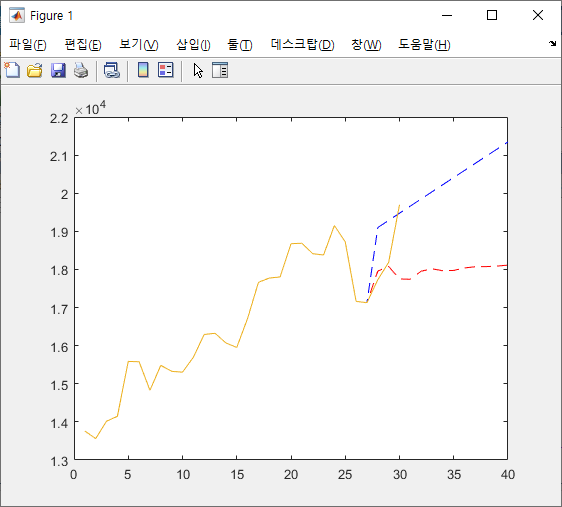
\includegraphics[width=0.5\linewidth]{fig1.PNG}
\end{center}
\caption{one of the main function result}
\label{fig:long}
\label{fig:onecol}
\end{figure}

\subsubsection{Autoregressive Model}\

\begin{lstlisting}[language=python, caption=AutoregressiveModel] 
function data = AutoregressiveModel(data, p, t)

X = [];
y = [];

for i = p+1:size(data,1)
    y = [y;data(i)];
    x = [];
    for j = 1:p
        x = [x, data(i-j)];
    end
    X = [X; [1, x]];
end

b = (transpose(X) * X)^(-1) * transpose(X) * y;
    
for i = 1:t
    x = [];
    for j = 0:p-1
        x = [x, data(end-j)];
    end
    
    y_ = [1, x] * b;
    
    data = [data; y_];
end

end
\end{lstlisting}

3번째 줄부터 13번째 줄은 주어진 데이터로부터 Y행렬과 X행렬을 구하는 과정이며, 15번째 줄을 통해 $\beta$ 행렬을 구한다.
이후 17번째줄부터 26번째 줄을 통해 t개의 예측값을 구해주는 코드이다.

\subsubsection{Gaussian Process}\

\begin{lstlisting}[language=python, caption=GaussianProcess]
function y = GaussianProcess(data, sig_f, sig_n, l, t)

n = size(data,1);
y = data;
x = transpose(1:n);

K = zeros(n,n);
for i = 1:n
    for j = 1:n
        K(i,j) = k(x(i), x(j), sig_f, sig_n, l);
    end
end

for i = 1:t
    xstar = n+i;
    Kstar = [];
    for j = 1:n
        Kstar = [Kstar, k(xstar, x(j), sig_f, sig_n, l)];
    end
        
    y_ = Kstar * K^(-1) * y(1:n);
    y = [y;y_];
end

end

function result = k(x, x_, sig_f, sig_n, l)

result = sig_f^2 * exp((-(x-x_)^2)/(2*l^2)) + sig_n^2*delta(x,x_);

end

function result = delta(x, x_)

if x == x_
    result = 1;
else
    result = 0;
end

end
\end{lstlisting}

위의 코드에서 3번째줄부터 12번째줄까지는 주어진 데이터를 통해 K행렬을 구하는 과정이며, 14번째줄부터 23번째줄까지는 예측값을 도출해내는 과정이다. 또한 27번째줄부터는 GaussianProcess 하는 과정에서 필요한 함수들을 정의해 놓은 것이다.

\subsection{실험 환경 및 실험}

먼저 운영체제는 Windows 10 환경에서 실험을 하였으며, MatLab은 R2020a버전을 사용하였다.

실험은 먼저 2020년 1월부터 11월까지의 비트코인 데이터와 2020년 11월 비트코인 데이터 2개의 데이터 셋을 가지고 실험을 하였으며, 주로 가장 적합한 파라미터 값을 찾기 위해 여려번의 실험을 하였다. 아래는 실험 과정에서 얻은 그래프들 중 일부이다.

노란 실선은 실제 데이터를, 빨간 점선은 AR 모델 예측값, 파란 점선은 GP 모델의 예측값을 의미한다.

\begin{figure}[h] %%% t: top, b: bottom, h: here
\begin{center}
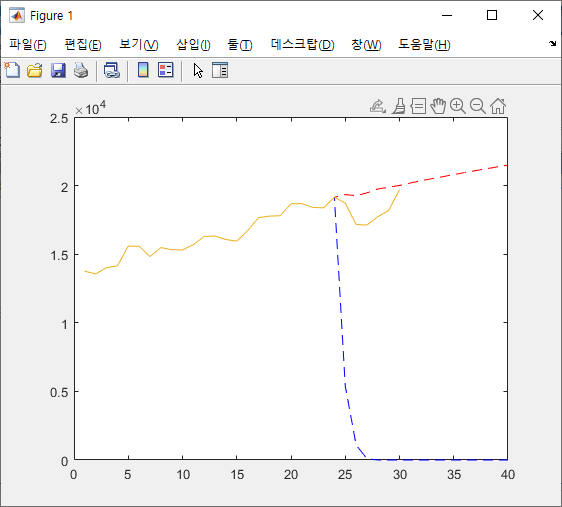
\includegraphics[width=0.5\linewidth]{fig2.PNG}
\end{center}
\caption{result1}
\label{fig:long}
\label{fig:onecol}
\end{figure}

\begin{figure}[h] %%% t: top, b: bottom, h: here
\begin{center}
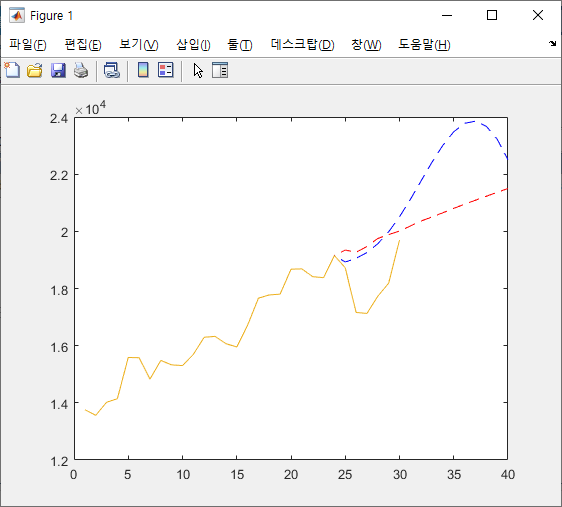
\includegraphics[width=0.5\linewidth]{fig3.PNG}
\end{center}
\caption{result2}
\label{fig:long}
\label{fig:onecol}
\end{figure}

\begin{figure}[h] %%% t: top, b: bottom, h: here
\begin{center}
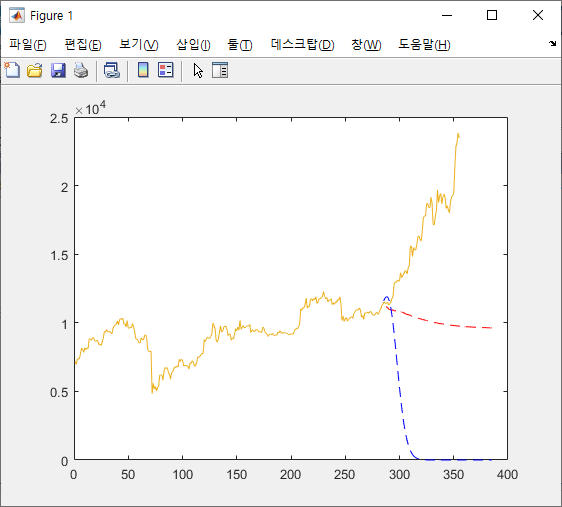
\includegraphics[width=0.5\linewidth]{fig4.PNG}
\end{center}
\caption{result3}
\label{fig:long}
\label{fig:onecol}
\end{figure}

\begin{figure}[h] %%% t: top, b: bottom, h: here
\begin{center}
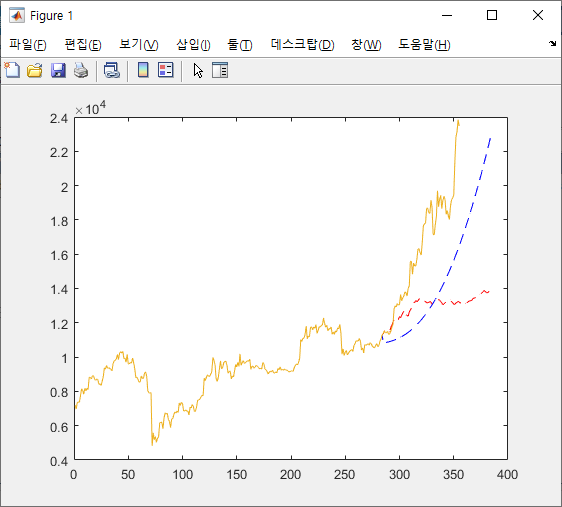
\includegraphics[width=0.5\linewidth]{fig5.PNG}
\end{center}
\caption{result4}
\label{fig:long}
\label{fig:onecol}
\end{figure}

\subsection{정보보안과 연결시키기 - 응용분야 도출}

Autoregressive의 경우 서버에 들어오는 패킷의 수에 대한 정보를 가지고 이후 이 서버에 얼만큼의 패킷이 들어오고 나가는지를 예측할 수 있을 것 같다. 나아가 공격 시도 등에 대한 정보들을 토대로 어느 시간대에 보안을 강화해야 하는지에 대한 정보도 예측할 수 있을 것 같다.

Gaussian Process의 경우 해킹을 시도한 나라와 그 위험도 등에 대한 정보를 분석하여 특정 국가에서 날아오는 네트워크 패킷이 얼마나 위험한지 등을 분석할 수 있을 것 같다.

\section{인공지능은 무엇인가}

한학기 동안 인공지능을 공부하면서 인공지능에 대한 생각이 많이 바뀌는 계기가 되었다. 수업을 듣기 전에는 인공지능이라고 하면 정말로 인간과 비슷한 사고를 하는 기계라고만 생각하였다. 인간의 지능, 생각을 따라한 것이 인공지능이라고 생각했던 것이다. 그러나 수업 시간 공부한 인공지능은 이런 것과 사뭇 거리가 있었다. 인간의 생각을 따라하는 분야만이 인공지능인 것이 아니라 인간의 특정 논리 회로를 모방한 모든 것이 인공지능에 포함되는 것이었다.

또한 인공지능을 직접 배우기 전에는 막연히 기술이 많이 발전하여 나도 나중에 인공지능을 쉽게 만들 수 있겠다고 생각하였는데, 수업 시간에 다양한 모델들이 나온 배경부터 그 과정까지 천천히 공부해보니 인공지능의 세계는 매우 넓고도 복잡하다고 생각하였다. 인공지능 수업을 들으면서 자연어 처리와 관련된 인공지능에도 관심이 생겨 RNN과 CNN 등 딥러닝에 대해 추가적으로 공부도 해 봤는데 이 또한 쉬운 과정이 아니었다. 그럼에도 불구하고 인공지능을 공부하면서 실제로 여러 프로그램을 짜보고 놀라운 결과를 얻어내는 과정을 통해 더욱 인공지능에 흥미가 생겼으며, 앞으로도 더 많은 모델들에 대해 공부해보고 싶다는 생각이 들었다.

\end{document}
\endinput
%%
%% End of file `sample-manuscript.tex'.
